\documentclass[reqno]{amsart}


\pagestyle{empty}

\usepackage{graphicx}
\usepackage[margin = 1cm]{geometry}
\usepackage{color}
\usepackage{cancel}
\usepackage{multirow}
\usepackage{framed}
\usepackage{amssymb}
\usepackage{stackengine}
\usepackage{tikz}

\newtheorem{thm}{Theorem}
\newtheorem{cor}{Corollary}
\theoremstyle{definition}
\newtheorem{definition}{Definition}

\newenvironment{handwave}{%
  \renewcommand{\proofname}{Handwavey proof}\proof}{\endproof}
  %\renewcommand{\qedsymbol}{$\blacksquare$}

\begin{document}
\begin{flushleft}
{\sc \Large AMATH 352 Rahman} \hfill Week 6
\bigskip
\end{flushleft}

\newcommand{\R}{\mathbb{R}}
\newcommand{\N}{\mathbb{N}}
\newcommand{\Z}{\mathbb{Z}}
\newcommand{\Q}{\mathbb{Q}}
\renewcommand{\CancelColor}{\color{red}}
\newcommand{\?}{\stackrel{?}{=}}
\renewcommand{\varphi}{\phi}
\newcommand{\card}{\text{Card}}
\newcommand{\bigzero}{\text{\Huge 0}}
\newcommand{\curvearrowdown}{{\color{red}\rotatebox{90}{$\curvearrowleft$}}}
\newcommand{\curvearrowup}{{\color{red}\rotatebox{90}{$\curvearrowright$}}}

\newcommand*\circled[1]{\color{red}\tikz[baseline=(char.base)]{
            \node[shape=circle,draw,inner sep=2pt] (char) {#1};}}



\section*{Sec. 2.5  The Fundamental Matrix Subspaces}

Consider the illustrative example matrix
%
\begin{equation*}
A = \begin{bmatrix}
1 & 2\\
1 & 2
\end{bmatrix} \longrightarrow U = \begin{bmatrix}
1 & 2\\
0 & 0
\end{bmatrix}
\end{equation*}

\underline{Row space}

The nonzero rows are a basis for the row space, and it has dimension $r$.  For the matrices above only
$\{(1, 2)\}$ is in the basis, and the dimension is $r=1$.  It should be noted that the basis isn't the row space;
the row space itself is $y = 2x$.

\underline{Nullspace}

So, we have one vector for the $2 \times 2$ matrix, but this only forms a $1-D$ space.
The nullspace is given by $x$ for the equation $Ax = 0 \Rightarrow Ux = 0$.  Then the basis for our
example is $\{(-2, 1)\}$ with a dimension of $m - r = 2 - 1 = 1$ where $m$ is the number of columns.
As with the row space, the nullspace itself is not the basis but rather the line $y = -x/2$.

\underline{Column space}

This is sometimes called the range.  The pivot columns of $U$ forms the basis for the column space of $U$
and the corresponding columns of $A$ form the column space of $A$.  Then the basis for the column space
of $U$ is $\{(1,0)\}$ and the basis for the column space of $A$ is $\{(1, 1)\}$.  The column space will
have the same dimension as the row space.

\underline{Left nullspace (null space of $A^T$)}

The left nullspace is just the nullspace of the transpose.  For our example the basis is $\{(1, -1)\}$
with a dimension of $n - r = 2 - 1 = 1$.  The left nullspace itself is $y = -x$.

\begin{thm}[Fundamental Theorem of Linear Algebra]
For an $n \times m$ matrix $A$,

\begin{enumerate}

\item  $\mathcal{C}(A)$ is the column space of $A$ and has dimension $r$.

\item  $\mathcal{N}(A)$ is the nullspace of $A$ and has dimension $m-r$.

\item  $\mathcal{C}(A^T)$ is the row space of $A$ and has dimension $r$.

\item  $\mathcal{N}(A^T)$ is the left nullspace of $A$ and has dimension $n-r$.

\end{enumerate}
\end{thm}

Here is a general picture of the subspaces (courtesy of Prof. Gilbert Strang - MIT Math):
%
\begin{figure}[htbp]
\centering
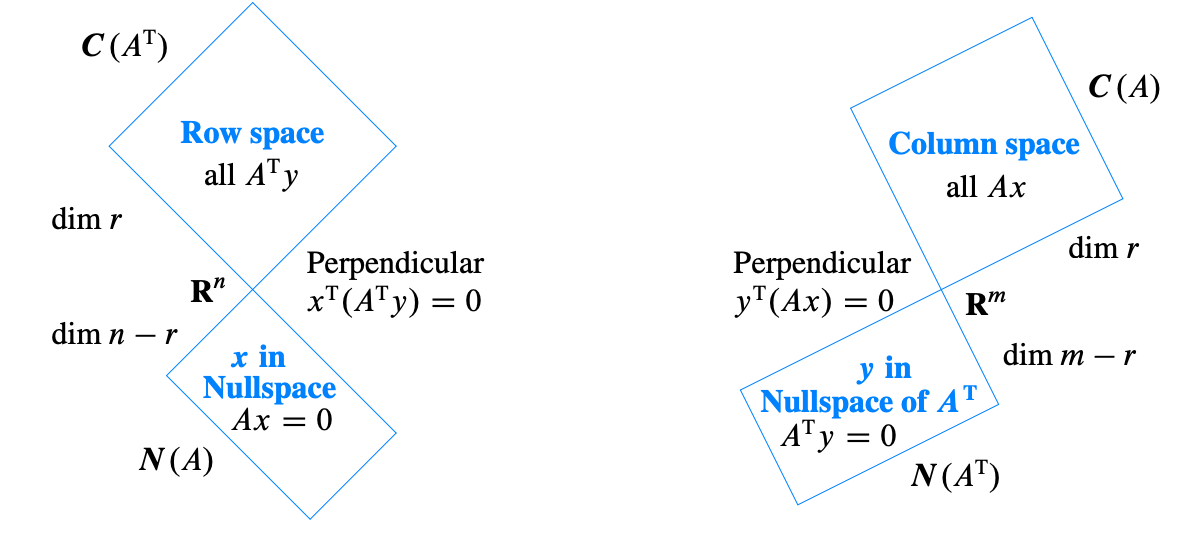
\includegraphics[width = 0.9\textwidth]{Subspaces}
\end{figure}

\pagebreak

Now lets do a bunch of examples.

\begin{enumerate}

\item[Ex:  ]  Find the basis for the row space of
%
\begin{equation*}
A = \begin{bmatrix}
1 & -3 & 2\\
4 & 2 & 1
\end{bmatrix}
\end{equation*}

\textbf{Solution:  }
Here we circle our pivots after we cannot reduce any further.
%
\begin{equation*}
U = \begin{bmatrix}
\circled{1} & -3 & 2\\
0 & \circled{14} & -7
\end{bmatrix}
\end{equation*}
%
and the basis is readily available:
%
\begin{equation*}
\left\lbrace \begin{pmatrix}
1\\
-3\\
2
\end{pmatrix}, \begin{pmatrix}
0\\
14\\
-7
\end{pmatrix}\right\rbrace
\end{equation*}
%
and it has a rank of $r = 2$ since it has two pivots.

\item[Ex:  ]  Find the basis for the row space of
%
\begin{equation*}
A = \begin{bmatrix}
1 & 6 & 18\\
7 & 40 & 116\\
-3 & -12 & -27
\end{bmatrix}
\end{equation*}

\textbf{Solution:  }
Again we eliminate and identify our pivots.
%
\begin{equation*}
\begin{bmatrix}
1 & 6 & 18\\
0 & -2 & -10\\
0 & 6 & 27
\end{bmatrix} \rightarrow \begin{bmatrix}
\circled{1} & 6 & 18\\
0 & \circled{-2} & -10\\
0 & 0 & \circled{-3}
\end{bmatrix}
\end{equation*}
%
Then the basis is
%
\begin{equation*}
\left\lbrace \begin{pmatrix}
1\\
6\\
18
\end{pmatrix}, \begin{pmatrix}
0\\
-2\\
-10
\end{pmatrix}, \begin{pmatrix}
0\\
0\\
-3
\end{pmatrix} \right\rbrace
\end{equation*}
%
and it has a rank of $r = 3$.

\item[Ex:  ]  Find the basis for the row space of
%
\begin{equation*}
A = \begin{bmatrix}
-2 & -4 & 4 & 3\\
3 & 6 & -6 ^ -4\\
-2 & -4 & 4 & 9
\end{bmatrix}
\end{equation*}

\textbf{Solution:  }
Again
%
\begin{equation*}
\begin{bmatrix}
-2 & -4 & 4 & 5\\
0 & 0 & 0 & 7/2\\
0 & 0 & 0 & 4
\end{bmatrix} \rightarrow \begin{bmatrix}
\circled{-2} & -4 & 4 & 5\\
0 & 0 & 0 & \circled{7/2}\\
0 & 0 & 0 & 0
\end{bmatrix}
\end{equation*}
%
and the basis is
%
\begin{equation*}
\left\lbrace \begin{pmatrix}
-2\\
-4\\
4\\
5
\end{pmatrix}, \begin{pmatrix}
0\\
0\\
0\\
7/2
\end{pmatrix}\right\rbrace
\end{equation*}
%
and the rank is $r=2$.

\end{enumerate}

You will notice that the vectors in the basis aren't unique.  As long as you can find vectors that
forms a basis that is all you need.

\begin{enumerate}

\item[Ex:  ]  Find the basis for the column space of
%
\begin{equation*}
A = \begin{bmatrix}
2 & 4\\
1 & 6
\end{bmatrix}
\end{equation*}

\textbf{Solution:  }
Since we want the basis for the column space of $A$ we must look back at the original matrix $A$.
When we eliminate we get
%
\begin{equation*}
\begin{pmatrix}
\circled{2} & 4\\
0 & \circled{4}
\end{pmatrix}
\end{equation*}
%
which means both columns of $A$ will be in the basis of the column space of $A$
%
\begin{equation*}
\left\lbrace \begin{pmatrix}
2\\
1
\end{pmatrix}, \begin{pmatrix}
4\\
6
\end{pmatrix}\right\rbrace
\end{equation*}
%
and the rank is $r = 2$.

\item[Ex:  ]  Find the basis for the column space of
%
\begin{equation*}
A = \begin{bmatrix}
1 & 2 & 4\\
-1 & 2 & 1
\end{bmatrix}
\end{equation*}

\textbf{Solution:  }
Again we want the basis of the column space of $A$, so we eliminate and find the pivot columns.
%
\begin{equation*}
\begin{pmatrix}
\circled{1} & 2 & 4\\
0 & \circled{4} & 5
\end{pmatrix}
\end{equation*}
%
so the basis of the column space of $A$ is
%
\begin{equation*}
\left\lbrace \begin{pmatrix}
1\\
-1
\end{pmatrix}, \begin{pmatrix}
2\\
2
\end{pmatrix}\right\rbrace
\end{equation*}
%
and the rank is $r = 2$.

Notice that the last column is not a pivot column.

\end{enumerate}

For the basis of a Null space we will do it through inspection here, but if you like you
should feel free to solve the $Ax=0$ problem for $x$.

\begin{enumerate}

\item[Ex:  ]  Find the basis for the Nullspace of
%
\begin{equation*}
A = \begin{bmatrix}
2 & -1\\
-6 & 3
\end{bmatrix}
\end{equation*}

\textbf{Solution:  }
To find the basis of the nullspace we eliminate then find the vectors $x$ that makes $Ax = 0$.
Elimination gives us
%
\begin{equation*}
\begin{bmatrix}
2 & -1\\
0 & 0
\end{bmatrix}
\end{equation*}
%
then the basis is
%
\begin{equation*}
\left\lbrace \begin{pmatrix}
1\\
2
\end{pmatrix}\right\rbrace
\end{equation*}

\item[Ex:  ]  Find the basis for the Nullspace of
%
\begin{equation*}
A = \begin{bmatrix}
1 & 2 & 3\\
0 & 1 & 0
\end{bmatrix}
\end{equation*}

\textbf{Solution:  }
Here we can find the basis straight away
%
\begin{equation*}
\left\lbrace \begin{pmatrix}
3\\
0\\
-1
\end{pmatrix}\right\rbrace
\end{equation*}

\item[Ex:  ]  Find the basis for the Nullspace of
%
\begin{equation*}
A = \begin{bmatrix}
1 & 2 & -3\\
2 & -1 & 4\\
4 & 3 & -2
\end{bmatrix}
\end{equation*}

\textbf{Solution:  }
We first do the elimination
%
\begin{equation*}
\begin{pmatrix}
1 & 2 & -3\\
0 & -5 & 10\\
0 & -5 & 10
\end{pmatrix} \rightarrow \begin{pmatrix}
1 & 2 & -3\\
0 & -5 & 10\\
0 & 0 & 0
\end{pmatrix}
\end{equation*}
%
Since there are three columns and two pivots, the nullspace will have a dimension of one, so the basis is
%
\begin{equation*}
\left\lbrace \begin{pmatrix}
-1\\
-2\\
1
\end{pmatrix}\right\rbrace
\end{equation*}

\item[Ex:  ]  Find the basis for the Nullspace of
%
\begin{equation*}
A = \begin{bmatrix}
5 & 2\\
3 & -1\\
2 & 1
\end{bmatrix}
\end{equation*}

\textbf{Solution:  }
We first eliminate
%
\begin{equation*}
\begin{pmatrix}
2 & 1\\
0 & -5/2\\
0 & -1/2
\end{pmatrix} \rightarrow \begin{pmatrix}
\circled{2} & 1\\
0 & \circled{-5/2}\\
0 & 0
\end{pmatrix}
\end{equation*}
%
Since it has two pivots and two columns $\dim(\mathcal{N}(A)) = 0$.

\item[Ex:  ]  Find the basis for the Nullspace of
%
\begin{equation*}
A = \begin{bmatrix}
1 & 3 & -2 & 4\\
0 & 1 & -1 & 2\\
-2 & -6 & 4 & -8
\end{bmatrix}
\end{equation*}

\textbf{Solution:  }
Next we have the row echelon matrix
%
\begin{equation*}
\begin{pmatrix}
\circled{1} & 3 & -2 & 4\\
0 & \circled{1} & -1 & 2\\
0 & 0 & 0 & 0
\end{pmatrix}
\end{equation*}
%
This has four columns and a rank of two, so the basis of the nullspace will consist of two vectors
%
\begin{equation*}
\left\lbrace \begin{pmatrix}
-1\\
1\\
1\\
0
\end{pmatrix}, \begin{pmatrix}
0\\
0\\
2\\
1
\end{pmatrix}\right\rbrace
\end{equation*}

Notice that the second vector here is different from the one in the recording.  Why is that?
Think about what the answer is and we can discuss it in the Zoom session.

\end{enumerate}



\end{document}